\begin{frame}
    \frametitle{\problemtitle}
    \begin{description}
        \item<+->[Problem:] On the fly, decide whether to use the \texttt{airline}
            or \texttt{buy} your own aircraft \\ and fly your\texttt{self}, keeping the cost below twice the optimum.
        \item<+->[Observation:] After \texttt{buy}ing your own aircraft, always fly your\texttt{self}.
        \item<+->[To solve:] When to \texttt{buy} your aircraft?
            \only<+->{$\Rightarrow$ ``\texttt{buy}'' when $b + cx < ax$.} \\
        \item<+->[Solution:] Print ``\texttt{airline}'' until the cost becomes higher than flying yourself. \\
            Then, print ``\texttt{buy}'', followed by printing ``\texttt{self}'' until you read ``\texttt{end}''.
        \item<+->[Edge cases:] $0 \leq a,b,c \leq 10^6$, so for example, it is possible that $a > b + c$ (immediately ``\texttt{buy}'') \\
            or $a = b = c = 0$ (always ``\texttt{airline}'').
        \item<+->[Note:] We did not specify the exact number of interactions up front. \\
            So, we check the cost condition after every \texttt{flight}.
    \end{description}
    \only<3-4>{
        \centering
        \vspace{-0.36\textheight}
        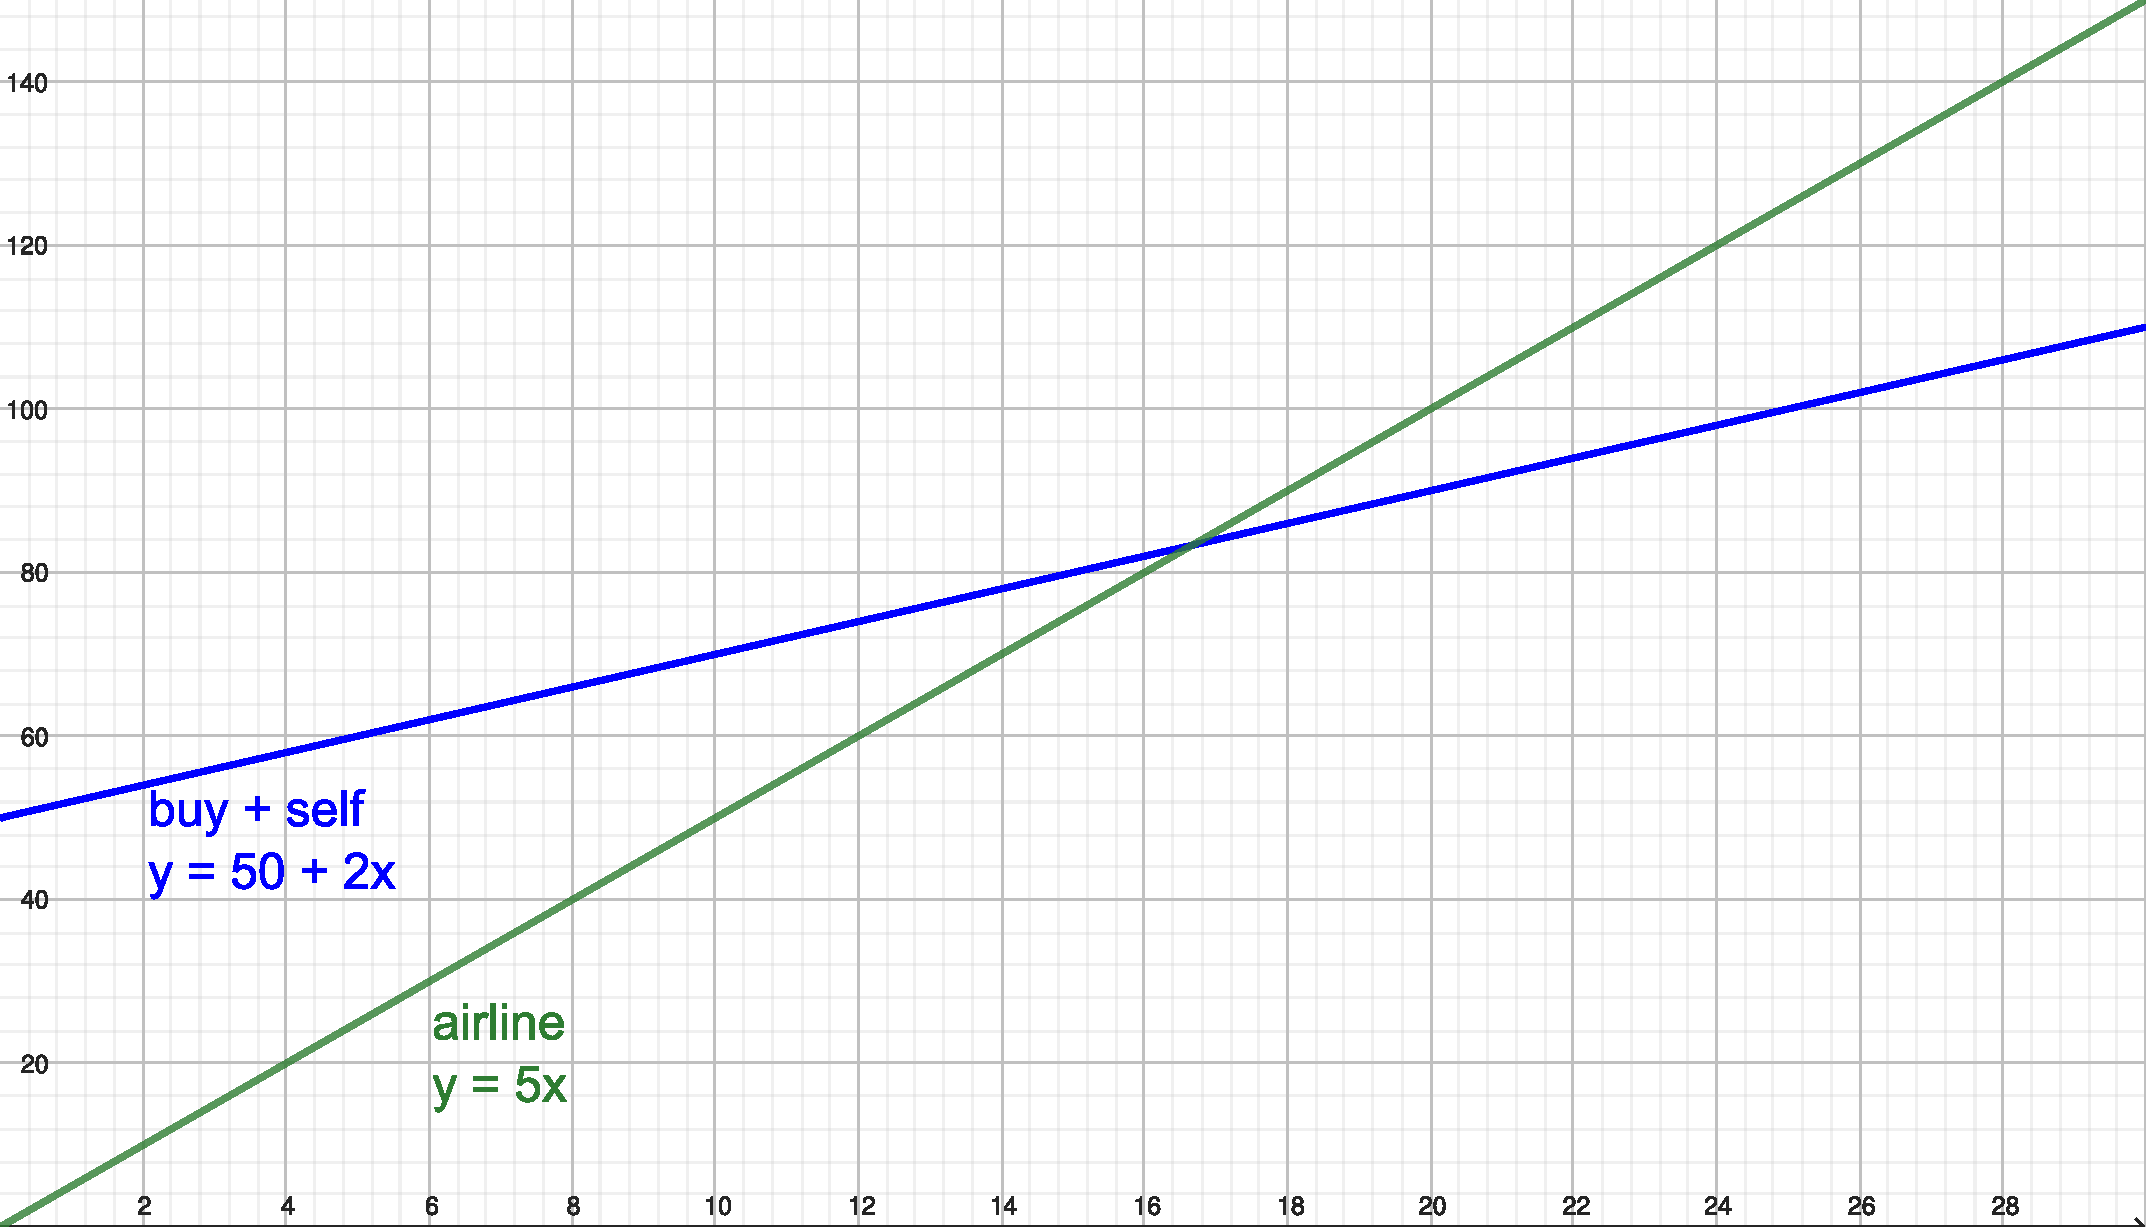
\includegraphics[height=0.55\textheight]{geogebra-graph}
        \small
        \vspace{-1.5em}
        ~\\
        \raggedleft
        \hspace{2em}
        Source: \href{https://www.geogebra.org/calculator}{Geogebra.org}
    }
    \only<5->\solvestats
\end{frame}
